\documentclass[tikz,border=1.35mm]{standalone}

\definecolor{splitred}{HTML}{AF2525}

% Face-based isotropic refinement skeleton for a general polyhedron.
% The four-valent apex produces a non-hexahedral child element after refinement.
\begin{document}
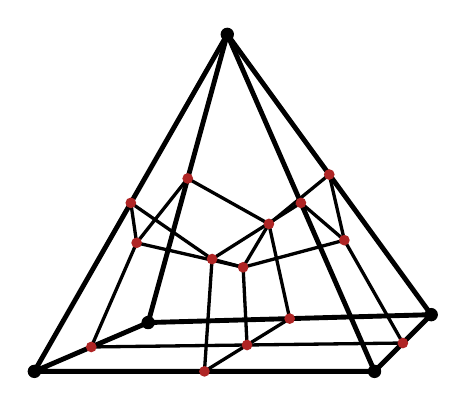
\begin{tikzpicture}[
  x={(18mm,0mm)},
  y={(7mm,4mm)},
  z={(0mm,18mm)},
  line join=round,
  line cap=round,
  edge/.style={draw=black,line width=0.62mm},
  split/.style={draw=black,line width=0.42mm}
]
  % Original vertices.
  \coordinate (v0) at (0,0,0);
  \coordinate (v1) at (2.4,0,0);
  \coordinate (v2) at (2.1,1.8,0);
  \coordinate (v3) at (0.2,1.55,0);
  \coordinate (apex) at (1.05,0.8,2.2);

  % Edge midpoints.
  \coordinate (m01) at (1.2,0,0);
  \coordinate (m12) at (2.25,0.9,0);
  \coordinate (m23) at (1.15,1.675,0);
  \coordinate (m30) at (0.1,0.775,0);
  \coordinate (m0a) at (0.525,0.4,1.1);
  \coordinate (m1a) at (1.725,0.4,1.1);
  \coordinate (m2a) at (1.575,1.3,1.1);
  \coordinate (m3a) at (0.625,1.175,1.1);

  % Face centroids and element centroid.
  \coordinate (fbase) at (1.175,0.8375,0);
  \coordinate (f01a) at (1.15,0.267,0.733);
  \coordinate (f12a) at (1.85,0.867,0.733);
  \coordinate (f23a) at (1.117,1.383,0.733);
  \coordinate (f30a) at (0.417,0.783,0.733);
  \coordinate (center) at (1.15,0.83,0.55);

  % Outer split topology.
  \draw[edge] (v0) -- (m01) -- (v1) -- (m12) -- (v2) -- (m23) -- (v3) -- (m30) -- cycle;
  \draw[edge] (apex) -- (m0a) -- (v0);
  \draw[edge] (apex) -- (m1a) -- (v1);
  \draw[edge] (apex) -- (m2a) -- (v2);
  \draw[edge] (apex) -- (m3a) -- (v3);

  % Face-centroid splits on the base and side faces.
  \draw[split] (fbase) -- (m01);
  \draw[split] (fbase) -- (m12);
  \draw[split] (fbase) -- (m23);
  \draw[split] (fbase) -- (m30);
  \draw[split] (center) -- (fbase);

  \draw[split] (f01a) -- (m01);
  \draw[split] (f01a) -- (m1a);
  \draw[split] (f01a) -- (m0a);
  \draw[split] (center) -- (f01a);

  \draw[split] (f12a) -- (m12);
  \draw[split] (f12a) -- (m2a);
  \draw[split] (f12a) -- (m1a);
  \draw[split] (center) -- (f12a);

  \draw[split] (f23a) -- (m23);
  \draw[split] (f23a) -- (m3a);
  \draw[split] (f23a) -- (m2a);
  \draw[split] (center) -- (f23a);

  \draw[split] (f30a) -- (m30);
  \draw[split] (f30a) -- (m0a);
  \draw[split] (f30a) -- (m3a);
  \draw[split] (center) -- (f30a);

  % Original vertices are black; refinement-created nodes are red.
  \foreach \p in {v0,v1,v2,v3,apex} {
    \fill[black] (\p) circle[radius=0.85mm];
  }
  \foreach \p in {m01,m12,m23,m30,m0a,m1a,m2a,m3a,
                  fbase,f01a,f12a,f23a,f30a,center} {
    \fill[splitred] (\p) circle[radius=0.68mm];
  }
\end{tikzpicture}
\end{document}
